\chapter{光子轨道、林德勒空间与史瓦西内部}

牛顿力学中的质点与史瓦西黑洞始于同一个理想化假设：所有产生引力的质量都集中在中心。然而，它们的中心却有着截然不同的含义。在牛顿力学中，即使只带有一点角动量的粒子也不会击中中心。而在黑洞中，一旦粒子越过视界，奇点就无法被避开。理解这一差异将带领我们依次考察圆轨道、光子球，最后是视界附近的一套新坐标。

\section{一个无法避开的中心}

真实的牛顿物质永远不会变成数学意义上的点。压强、材料强度以及其他力都会抵抗压缩。即使我们仍然用质点作为理想化模型，下落的粒子也很少会击中它。一条严格径向的轨迹可以到达\(r=0\)，但哪怕最微小的横向速度也会提供角动量。离心势垒随后使粒子绕中心转过而远离。

广义相对论改变了结论。一个足够致密的物体可以形成黑洞，而黑洞内部通过绕开中心的方式挫败了牛顿式的逃逸。原因比“力更强”更为深刻：在视界内部，\(r\)的减小是一个未来方向。我们将逐步抵达这一陈述，而不是直接假设它。

\begin{classroomqa}
\audiencequestion{牛顿力学中难以击中中心，是否仅仅是把两个物体都当作点来处理的后果？}
\lecturerresponse{点的理想化是比较的一部分，但并非全部区别所在。在牛顿力学中，任何非零角动量都使轨道绕过该点。在相对论性内部，奇点位于每一条下落类时轨迹的未来；角向运动无法提供逃逸。
\lecturetimestamp{00:04:52--00:05:13}}
\end{classroomqa}

\section{视界与奇点}

我们暂时把史瓦西几何视为已知：
\begin{equation}
d\tau^{2}
=
\left(1-\frac{2MG}{r}\right)dt^{2}
-
\frac{dr^{2}}{1-\frac{2MG}{r}}
-
r^{2}d\Omega^{2}.
\label{eq:l6-schwarzschild}
\end{equation}
选出这一度规的场方程将在后面出现。我们当前的任务是了解该度规告诉我们什么。

单位球面上的度规可以写成
\begin{equation}
d\Omega^{2}
=d\vartheta^{2}+\cos^{2}\vartheta\,d\phi^{2}
\label{eq:l6-angular-metric}
\end{equation}
其中\(\vartheta\)是从赤道面量起的纬度。若改用更常见的从轴量起的极角，则余弦变为正弦。球对称性使每一条轨道都可以置于一个固定平面内，因此在下面的计算中只有一个角坐标会保留下来。

\begin{figure}[htbp]
\centering
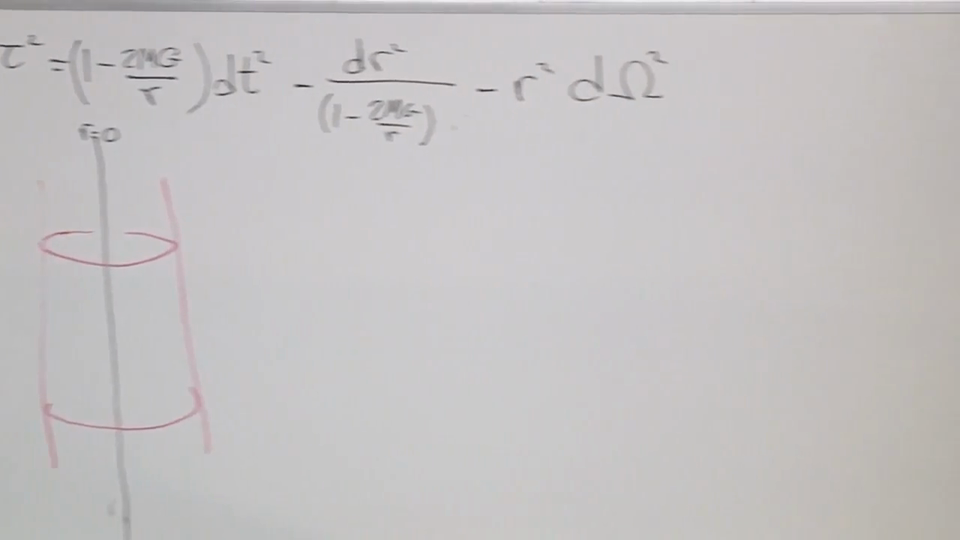
\includegraphics[width=0.88\textwidth]{lecture_06_figure_01.png}
\caption{史瓦西度规与曲面\(r=2MG\)的柱状时空图像。中心线是\(r=0\)；红色柱面是史瓦西坐标中的视界。}
\lectureframe{00:09:45}
\end{figure}

远离源处，\(2MG/r\)很小，式~\eqref{eq:l6-schwarzschild}趋近于球坐标中的闵可夫斯基度规。有两个半径格外突出：
\begin{equation}
r=2MG,
\qquad
r=0.
\end{equation}
它们绝不能被混淆。在\(r=2MG\)处，\(dt^{2}\)的系数为零，而\(dr^{2}\)的系数发散。史瓦西坐标系已经变得奇异。曲率本身在那里仍然有限。相反，在\(r=0\)处，曲率不变量发散。潮汐场沿径向拉伸一个延展物体，并沿横向无限制地挤压它。那是物理奇点，而不是坐标的缺陷。

\subsection{为下落计时的两种方式}

对于视界外的一个静止时钟，
\begin{equation}
d\tau
=
\sqrt{1-\frac{2MG}{r}}\,dt.
\label{eq:l6-static-clock}
\end{equation}
在\(r\)很大时，\(d\tau\simeq dt\)。在视界附近，保持在固定\(r\)处的时钟的固有时相对于远处所保持的史瓦西时间推进得极其缓慢。

同一组坐标把径向下落描述为需要\(t\)取无穷大值才能到达\(r=2MG\)。下落者自身所经历的固有时是有限的。这些陈述之间没有矛盾。下落者携带的时钟测量的是沿其世界线的固有时。它可以是机械钟、由米尺两端镜子构成的光钟、一次心跳，或大脑中物理过程的相继发生。这些都不测量远处的坐标\(t\)。两个时钟之间的区别将在近视界图中变得可见。

\section{由固有时作用量得到的圆运动}

在回到下落问题之前，让我们先解决另一个问题：在什么条件下，一个有质量粒子或一个光子能够环绕黑洞运行？计算从与任何自由运动的相对论粒子相同的作量原理开始，
\begin{equation}
S=-m\int d\tau.
\label{eq:l6-particle-action}
\end{equation}
光会被地球弯曲，但地球的场远不足以强到把一条光线闭合成轨道。地球的施瓦西半径只有大约一厘米的量级。人们必须把整个地球压缩到大致这个尺度，约一颗小坚果的大小，强场问题才会变得相关。

令 \(c=1\)，把运动限制在一个赤道平面内，并定义
\begin{equation}
F(r)=1-\frac{2MG}{r},
\qquad
G(r)=\frac{1}{F(r)}.
\label{eq:l6-fg}
\end{equation}
使用坐标时 \(t\) 作为参数，得到
\begin{equation}
d\tau
=dt\sqrt{F-G\dot r^{\,2}-r^{2}\dot\theta^{\,2}},
\end{equation}
因此
\begin{equation}
\mathcal L
=
-m\sqrt{F-G\dot r^{\,2}-r^{2}\dot\theta^{\,2}}.
\label{eq:l6-lagrangian}
\end{equation}
因子 \(m\) 使作用量具有通常的能量乘时间的量纲。

\begin{figure}[htbp]
\centering
\includegraphics[width=0.76\textwidth]{lecture_06_figure_02.png}
\caption{正在黑板上组装平方根粒子拉格朗日量。完整表达式见式 ~\eqref{eq:l6-lagrangian}。}
\lectureframe{00:31:53}
\end{figure}

对于任意广义坐标 \(q\)，
\begin{equation}
p_q=\frac{\partial\mathcal L}{\partial\dot q}.
\end{equation}
把 \(\mathcal L\) 保留给拉格朗日量、把 \(L\) 保留给角动量是有用的。令
\begin{equation}
\Delta=F-G\dot r^{\,2}-r^{2}\dot\theta^{\,2},
\end{equation}
两个动量是
\begin{align}
L=p_\theta
&=\frac{mr^{2}\dot\theta}{\sqrt{\Delta}},
\label{eq:l6-angular-momentum}\\
p_r
&=\frac{mG\dot r}{\sqrt{\Delta}}.
\label{eq:l6-radial-momentum}
\end{align}
径向动量不守恒，因为径向坐标出现在拉格朗日量中。角度 \(\theta\) 不出现，所以 \(L\) 守恒。

在 \(\mathcal L\) 中也没有显含的 \(t\)。因此哈密顿量守恒：
\begin{align}
E=H
&=p_r\dot r+L\dot\theta-\mathcal L \\
&=\frac{mG\dot r^{\,2}}{\sqrt{\Delta}}
  +\frac{mr^{2}\dot\theta^{\,2}}{\sqrt{\Delta}}
  +m\sqrt{\Delta} \\
&=\frac{mF}{\sqrt{\Delta}}.
\label{eq:l6-energy-general}
\end{align}
这是力学的一种典型节律。一个原理给出作用量；一次计算给出动量；对称性随后把计算转回能量守恒和角动量守恒的原理。人们本可以立即求解所有欧拉--拉格朗日方程，但由旋转对称性和时间平移对称性提供的常量消除了其中大量工作。

\subsection{圆轨道能量}

对于圆轨道，
\begin{equation}
\dot r=0.
\end{equation}
引入单位质量的角动量，
\begin{equation}
\lambda=\frac{L}{m}.
\end{equation}
方程 ~\eqref{eq:l6-angular-momentum} 和
\eqref{eq:l6-energy-general} 变为
\begin{align}
\lambda
&=\frac{r^{2}\dot\theta}
{\sqrt{F-r^{2}\dot\theta^{\,2}}},
\label{eq:l6-lambda-circular}\\
E
&=\frac{mF}{\sqrt{F-r^{2}\dot\theta^{\,2}}}.
\label{eq:l6-energy-circular-first}
\end{align}

\begin{figure}[htbp]
\centering
\includegraphics[width=0.82\textwidth]{lecture_06_figure_04.png}
\caption{圆 Schwarzschild 运动的约化角动量和能量。首先使用角动量方程从能量中消去 \(\dot\theta\)。}
\lectureframe{00:39:14}
\end{figure}

将式 ~\eqref{eq:l6-lambda-circular} 平方并解出角速度，得到
\begin{equation}
\dot\theta^{\,2}
=
\frac{\lambda^{2}F}
{r^{2}\left(r^{2}+\lambda^{2}\right)}.
\label{eq:l6-angular-speed}
\end{equation}
代入式 ~\eqref{eq:l6-energy-circular-first} 后，剩下的能量只依赖于所提议的半径和固定的角动量：
\begin{equation}
E(r,\lambda)
=m\sqrt{F(r)}\,\frac{\sqrt{r^{2}+\lambda^{2}}}{r}.
\label{eq:l6-circular-energy}
\end{equation}

课堂上暂停下来作一个牛顿力学的比较。在普通圆轨道中，角频率和切向速率随半径增大而减小，但角动量包含一个半径因子。因此，人们不应仅从角速率推断 \(L\) 的行为。相对论公式把这些因子明确保留下来。

\section{光的圆轨道}

光子具有能量和动量，尽管其静质量为零。因此，式 ~\eqref{eq:l6-circular-energy} 的无质量极限必须小心取。如果 \(m\) 在固定 \(\lambda\) 下趋于零，那么 \(L=m\lambda\) 也会趋于零。相反，取
\begin{equation}
m\longrightarrow0,
\qquad
\lambda\longrightarrow\infty,
\qquad
L=m\lambda\ \text{fixed}.
\label{eq:l6-massless-limit}
\end{equation}
于是 \(\lambda^{2}\) 项占主导，光子能量变为
\begin{equation}
E_\gamma(r;L)
=L\,\frac{\sqrt{1-\frac{2MG}{r}}}{r}.
\label{eq:l6-photon-energy}
\end{equation}
因子 \(L\) 乘在整个径向函数上。它影响能量标度，但不影响圆轨道的半径。

\begin{figure}[htbp]
\centering
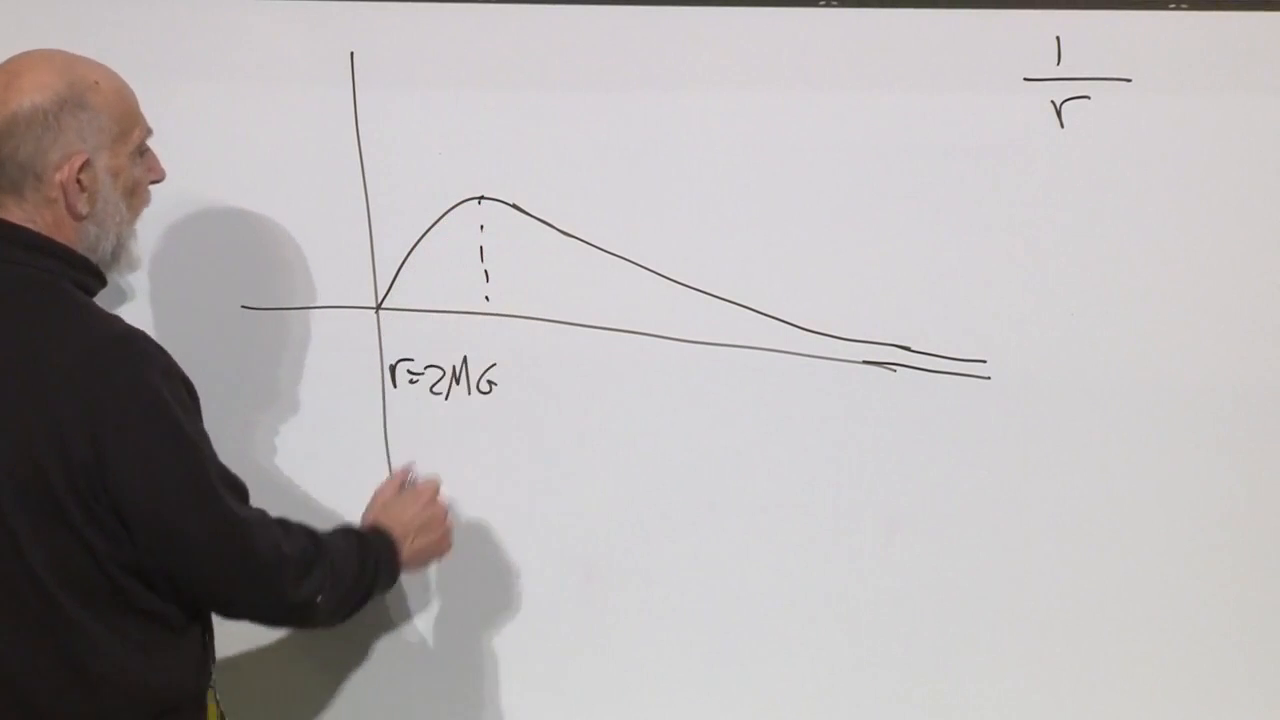
\includegraphics[width=0.88\textwidth]{lecture_06_figure_05.png}
\caption{光子能量中的径向因子。它在地平线处为零，在大半径处趋于零，并在两者之间有一个极大值。}
\lectureframe{00:50:50}
\end{figure}

在固定 \(L\) 下，径向平衡要求一个驻点：
\begin{equation}
\frac{d}{dr}
\left[
\frac{\sqrt{1-\frac{2MG}{r}}}{r}
\right]=0.
\end{equation}
求导，
\begin{equation}
-\frac{\sqrt{1-\frac{2MG}{r}}}{r^{2}}
+
\frac{MG}
{r^{3}\sqrt{1-\frac{2MG}{r}}}
=0,
\end{equation}
因此
\begin{equation}
r=3MG.
\label{eq:l6-photon-sphere}
\end{equation}
这个半径是施瓦西半径的一倍半。它通常被称为光子球。

该驻点是极大值，所以圆形光子轨道是不稳定的。恰好放在 \(3MG\) 处的光子会留在那里。任意小的径向位移最终都会把它从极大值处送走。恰好在光子球外侧，一条光线可以扫过非常大的角度，也许在逃逸前绕黑洞转许多圈。恰好在它内侧，一条近乎切向的光线可以绕几圈，然后穿过地平线落入。

\begin{figure}[htbp]
\centering
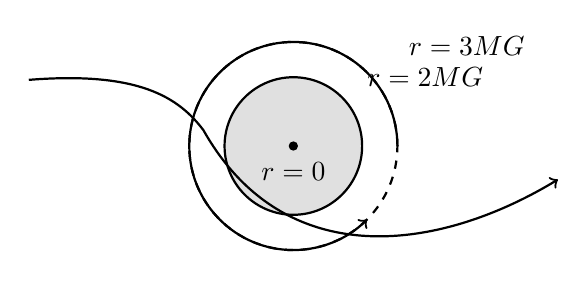
\begin{tikzpicture}[scale=1.12]
\fill[black!12] (0,0) circle (0.78);
\draw[thick] (0,0) circle (0.78);
\draw[dashed,thick] (0,0) circle (1.18);
\fill (0,0) circle (1.5pt);
\draw[->,thick] (1.18,0) arc (0:315:1.18);
\draw[->,thick] (-3.0,0.75)
  .. controls (-1.75,0.85) and (-1.30,0.55) .. (-1.02,0.18)
  .. controls (-0.10,-1.45) and (1.65,-1.20) .. (3.0,-0.38);
\node[right] at (0.73,0.78) {\(r=2MG\)};
\node[right] at (1.20,1.13) {\(r=3MG\)};
\node[below] at (0,-0.08) {\(r=0\)};
\end{tikzpicture}
\caption{地平线、光子球和一条强偏折光线。任意接近不稳定圆轨道的光线在逃逸或向内落入之前，可以累积任意大的偏折。}
\end{figure}

\begin{classroomqa}
\audiencequestion{为什么要固定角动量，它与光子的频率和入射轨迹有何关系？}
\lecturerresponse{每条光线都携带一个关于黑洞守恒的角动量。其频率决定了线动量的大小，而它偏离中心的距离则有助于确定\(L\)。在圆轨道之外，半径和角动量可以独立选取。要求光子作圆轨道运动，就把运动与唯一的半径\(3MG\)联系起来，而式~\eqref{eq:l6-photon-energy}中的因式分解表明，该半径与\(L\)的大小无关。
\lecturetimestamp{00:54:43--00:57:02}}
\end{classroomqa}

\begin{classroomqa}
\audiencequestion{为什么能量的极大值能确定一条轨道？}
\lecturerresponse{在固定\(L\)消去角向运动之后，剩下的函数起着有效径向能量的作用。驻点给出径向平衡。若是最小值则稳定；而此点是极大值，因此给出不稳定的圆轨道。称它既是平衡的又是不稳定的，这并不矛盾。
\lecturetimestamp{00:57:51--00:58:54}}
\end{classroomqa}

有质量粒子可以在\(3MG\)之外拥有类时圆轨道，不过最靠近光子球的那几条是不稳定的。无质量粒子只有位于\(3MG\)处的圆轨道。在光子球内部，切向运动的光子会向内坠落；运动更慢的物体维持这种轨道的机会也不会更好。这一陈述针对的是角向运动。在视界之外，即使其起始半径低于\(3MG\)，一条足够朝外的光线仍能逃逸。

\section{黑洞对图像做了什么}

光子球解释了为什么黑洞不仅仅是一个贴在原本不变的天空上的暗盘。来自背景天体的光可以沿多条路径到达观测者。一条光线可以从黑洞的一侧经过，另一条从另一侧经过，还有别的光线可能绕黑洞一圈或更多圈。结果可能包含位移的像、重复的像、环，以及与额外绕行圈数相关的无限序列的越来越精细、越来越暗淡的像。确切的图像很复杂，但其起源已经包含在那条不稳定轨道之中。

当光源、透镜和观测者足够对齐时，像可以形成爱因斯坦环。引力透镜环在自然界中已被观测到。完整的黑洞图像需要对许多初始方向积分零测地线，这是一项很适合计算机的计算。

\begin{classroomqa}
\audiencequestion{这个光学边界指的是光子球还是视界？}
\lecturerresponse{它们扮演不同的角色。位于\(2MG\)的视界是因果边界：没有任何指向未来的信号能从其内部逃逸。位于\(3MG\)的光子球控制切向运动和强透镜效应。在这两个半径之间，一条朝外的径向光线可以逃逸，而一条切向光线则会落入。介于两者之间的方向可能先绕行，然后逃逸或被捕获。
\lecturetimestamp{01:02:47--01:03:40}}
\end{classroomqa}

\begin{classroomqa}
\audiencequestion{一般的光线路径能否被计算出来，而不仅仅是画个草图？}
\lecturerresponse{可以。把零条件代入测地线方程或欧拉--拉格朗日方程，并用选定的初始数据积分。这些方程在概念上并不新鲜，但光线追踪在代数上很繁琐，这就是为什么数值计算是获得图像的实际方法。
\lecturetimestamp{01:03:48--01:04:27}}
\end{classroomqa}

\begin{classroomqa}
\audiencequestion{直接应用欧拉--拉格朗日方程会使圆轨道的计算更难吗？}
\lecturerresponse{它会给出相同的结果。无论用哪种方法，作用量都是恰当的出发点，但循环坐标暴露出守恒的能量和角动量。先使用这些常量是通向圆轨道条件的更短路径。
\lecturetimestamp{01:04:33--01:05:49}}
\end{classroomqa}

\section{近视界度规是林德勒空间}

现在我们回到视界。史瓦西系数在那里似乎发散或消失，而穿过视界时它们的符号互换。然而，下落的观测者在那个表面上并不会遇到发散的局部曲率。等效原理告诉我们这两种说法如何能同时成立。

从二维闵可夫斯基时空开始：
\begin{equation}
d\tau^{2}=dT^{2}-dX^{2}.
\end{equation}
在右林德勒楔形区中定义
\begin{equation}
X=\rho\cosh\omega,
\qquad
T=\rho\sinh\omega.
\label{eq:l6-rindler-map}
\end{equation}
\(\rho\)为常数的曲线满足
\begin{equation}
X^{2}-T^{2}=\rho^{2},
\end{equation}
所以它们是双曲线，即匀加速观测者的世界线。把式~\eqref{eq:l6-rindler-map}代入平坦度规得到
\begin{equation}
d\tau^{2}
=\rho^{2}d\omega^{2}-d\rho^{2}.
\label{eq:l6-rindler-metric}
\end{equation}
现在令
\begin{equation}
\rho^{2}=4\xi,
\qquad
\omega=\frac{t}{2}.
\label{eq:l6-rindler-rescale}
\end{equation}
由于\(d\rho^{2}=d\xi^{2}/\xi\)，式~\eqref{eq:l6-rindler-metric}变为
\begin{equation}
d\tau^{2}
=\xi\,dt^{2}-\frac{d\xi^{2}}{\xi}.
\label{eq:l6-xi-metric}
\end{equation}

\begin{classroomqa}
\audiencequestion{角向坐标或横向坐标到哪里去了？}
\lecturerresponse{它们只是被隐去了。我们正在考察包含穿越视界行为的局部 \(t\)-\(r\) 平面。两个横向方向仍然规则，可以恢复；它们不改变正在分析的坐标奇点。
\lecturetimestamp{01:16:27--01:16:47}}
\end{classroomqa}

为了与施瓦茨席尔德度规比较，选取 \(2MG=1\) 的单位。式~\eqref{eq:l6-schwarzschild}的径向部分为
\begin{equation}
d\tau^{2}
=
\frac{r-1}{r}\,dt^{2}
-
\frac{r}{r-1}\,dr^{2}.
\end{equation}
在 \(r=1\) 附近，小量分子 \(r-1\) 必须保留，而原本无害的 \(r\) 因子可以替换为 1。因此
\begin{equation}
d\tau^{2}
\simeq
(r-1)\,dt^{2}
-
\frac{dr^{2}}{r-1}.
\end{equation}
令
\begin{equation}
\xi=r-1,
\end{equation}
这恰好就是式~\eqref{eq:l6-xi-metric}。近视界施瓦茨席尔德几何在局部就是平直时空的 Rindler 描述。

\begin{classroomqa}
\audiencequestion{如果底层时空是平直的，这些怎么可能是加速坐标？}
\lecturerresponse{加速度属于观测者，而不一定属于曲率。固定 \(\rho\) 的世界线在闵可夫斯基时空中是匀加速的。同样，在黑洞附近被保持在固定半径处的观测者必须被支撑以抵抗自由下落。等效原理使局部描述一致，尽管完整的施瓦茨席尔德时空是弯曲的。
\lecturetimestamp{01:22:19--01:24:06}}
\end{classroomqa}

\section{穿越 Rindler 视界}

右楔公式只覆盖 \(\xi>0\)：
\begin{equation}
X=2\sqrt{\xi}\cosh\frac{t}{2},
\qquad
T=2\sqrt{\xi}\sinh\frac{t}{2}.
\label{eq:l6-rindler-outside}
\end{equation}
曲面 \(\xi=0\) 是零线 \(X=T\)。为了延续到未来楔，令
\begin{equation}
\zeta=-\xi>0
\end{equation}
并交换双曲角色：
\begin{equation}
T=2\sqrt{\zeta}\cosh\frac{t}{2},
\qquad
X=2\sqrt{\zeta}\sinh\frac{t}{2}.
\label{eq:l6-rindler-inside}
\end{equation}
度规仍然是
\begin{equation}
d\tau^{2}
=\xi\,dt^{2}-\frac{d\xi^{2}}{\xi},
\end{equation}
但当 \(\xi<0\) 时，\(dt^{2}\) 的系数为负，而 \(d\xi^{2}\) 的系数为正。坐标 \(\xi\)，因而施瓦茨席尔德径向方向，已经变成类时的；\(t\) 已经变成类空的。

\begin{figure}[htbp]
\centering
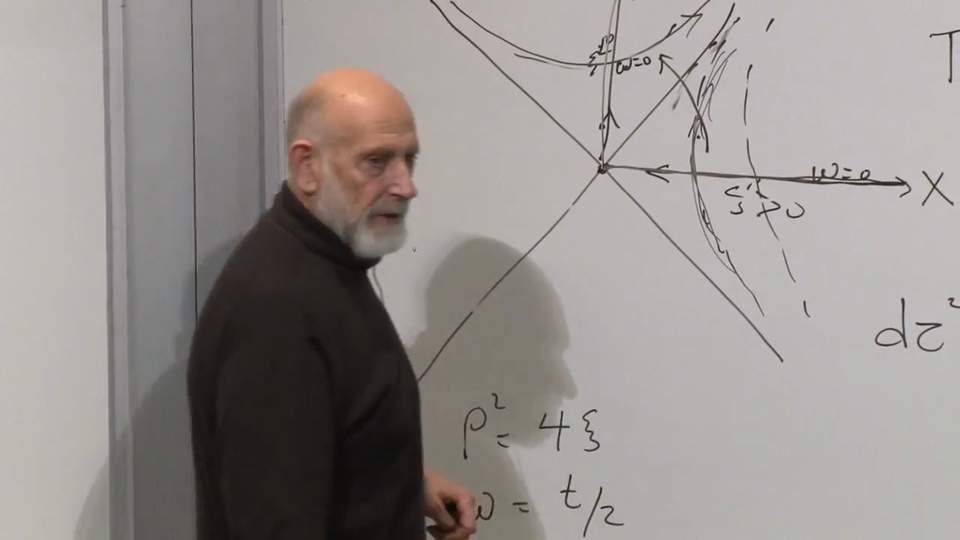
\includegraphics[width=0.88\textwidth]{lecture_06_figure_06.png}
\caption{Rindler 楔、它们的零边界，以及从 \(\xi>0\) 到 \(\xi<0\) 的延续。黑板上还记录了 \(\rho^{2}=4\xi\) 和 \(\omega=t/2\)。}
\lectureframe{01:29:40}
\end{figure}

\begin{classroomqa}
\audiencequestion{这幅坐标图中的某些曲线会运动得比光还快吗？}
\lecturerresponse{坐标网格线不必是物质客体的世界线。它的坐标斜率可以看起来超光速，而不违反因果性。物理光线仍然位于零线上，物理粒子仍然位于其局部光锥之内。
\lecturetimestamp{01:28:44--01:29:08}}
\end{classroomqa}

继续深入施瓦茨席尔德内部，最终会把我们带到 \(r=0\)。那个边界是类空的。因此，把它描述为时间比描述为地点更恰当：黑洞内部每一条未来指向的类时或零轨迹都会到达它。人可以绕过一个地点。人不能绕过自己的未来。

\begin{classroomqa}
\audiencequestion{图能否简单地穿过 \(r=0\) 延续到负 \(r\)，而 \(r=0\) 仍然是中心吗？}
\lecturerresponse{坐标图可能诱使我们将一条线延长，但经典施瓦茨席尔德解终止于曲率奇点。\(r=0\) 仍然可以称为中心，但它是一个非常不寻常的中心：在内部，它是一个类空的未来边界。不存在穿过它到达负半径区域的规则通道。
\lecturetimestamp{01:32:16--01:34:06}}
\end{classroomqa}

\begin{classroomqa}
\audiencequestion{Rindler 图中的对角轴是类光的吗，并且下落者能在加速时间的有限值处进入吗？}
\lecturerresponse{是的，楔边界是零线。自由下落的世界线在一个普通的有限事件处、在有限固有时内穿过这样一条线。加速坐标 \(t\)，或等价地 \(\omega\)，在外部固定 \(\rho\) 描述中无界地延伸；变得无限的是那个坐标赋值，而不是穿越事件。
\lecturetimestamp{01:34:26--01:35:03}}
\end{classroomqa}

\section{外部的 Alice 与下落的 Bob}

让 Alice 保持在外部固定半径处，被支撑以抵抗引力，并让 Bob 自由下落。在视界附近，Alice 沿着一条类似 Rindler 的双曲线运动。她的固定 \(t\) 切片越来越密集地逼近零边界。Bob 世界线上每一个被 Alice 标以有限 \(t\) 的事件都位于视界之外，因此她从未给他的穿越赋予有限的施瓦茨席尔德时间。

Bob 携带一个固有时钟。他的轨迹在那个时钟的有限间隔内穿过零线。当他穿过时，局部没有发生任何发散的事情。视界在全局上是决定性的，但在局部是普通的。

\begin{figure}[htbp]
\centering
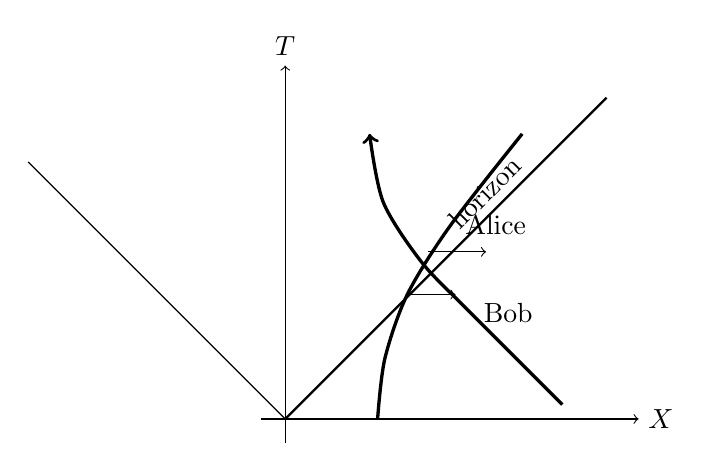
\begin{tikzpicture}[scale=1.02]
\draw[->] (-0.3,0) -- (4.4,0) node[right] {\(X\)};
\draw[->] (0,-0.3) -- (0,4.4) node[above] {\(T\)};
\draw[thick] (0,0) -- (4.0,4.0);
\draw[thin] (0,0) -- (-3.2,3.2);
\node[rotate=45,above] at (2.65,2.65) {horizon};
\draw[very thick]
  plot[smooth] coordinates {(1.15,0.0) (1.24,0.75) (1.52,1.55)
  (2.05,2.40) (2.95,3.55)};
\node[right] at (2.12,2.42) {Alice};
\draw[very thick,->]
  plot[smooth] coordinates {(3.45,0.18) (2.85,0.78) (2.25,1.38)
  (1.70,1.95) (1.22,2.70) (1.05,3.55)};
\node[right] at (2.35,1.32) {Bob};
\draw[->] (1.52,1.55) -- (2.12,1.55);
\draw[->] (1.78,2.08) -- (2.50,2.08);
\end{tikzpicture}
\caption{Alice 的加速外部世界线与 Bob 的自由下落世界线。Alice 的坐标切片逼近视界；Bob 在有限固有时内穿过它。}
\end{figure}

\begin{classroomqa}
\audiencequestion{当Bob回头看向Alice时，他看到了什么？穿越之后他的时钟又会怎样？}
\lecturerresponse{Bob看到Alice以维持她留在外部所需的加速度远离，但他并未在自己的穿越处看到一个奇异事件。Alice可以被支撑在固定半径处；轨道则是另一种可能的设置。Bob的时钟继续正常地测量他的固有时\(\tau\)。在内部，说径向坐标是类时的，描述的是因果几何；这并不会真的把他的手表变成一把米尺。他的世界线最终终止于\(r=0\)。
\lecturetimestamp{01:39:51--01:44:45}}
\end{classroomqa}

现在这条零线被认作视界本身，而不仅仅是一个坐标系数表现失常的点。在它外部，一族径向光线向外运动。在它内部，两个未来光锥方向都指向更小的\(r\)。每一条指向未来的有质量轨迹都必须保持在这些零方向之间，因此会到达奇点。

\section{信号、红移与正在形成的视界}

假设坍缩的物质发出一系列规则的光脉冲。远处的观测者接收到后续脉冲的间隔越来越长。它们的频率从光学波段移向红外、微波、射电以及更长的波长。在一个理想化的经典计算中，外部观测者可以继续把越来越晚的信号与接近视界的物质联系起来，但在实践中，源会迅速变得过于红移、过于微弱而无法探测。

\begin{classroomqa}
\audiencequestion{在坍缩过程中，外部观测者是否看到所有物质干脆冻结在视界处？}
\lecturerresponse{在Schwarzschild时间中，坍缩物质的表面渐近地接近视界，并显得越来越冻结。实际被观测到的内容编码在光信号中，而这些信号变得越来越延迟、越来越红移、越来越微弱。这种坐标描述并没有说下落的物质经历了无限长的固有时。
\lecturetimestamp{01:47:06--01:48:11}}
\end{classroomqa}

\begin{classroomqa}
\audiencequestion{一个足够晚的观测者能否恢复整个下落的历史？}
\lecturerresponse{只能通过那些已经发出并设法到达观测者的信号。相继的脉冲越来越彼此分离，并且越来越红移。一个具有无限灵敏度的理想观测者可以沿着经典信号追踪到越来越长的波长；而一个实际的观测者则看到该物体逐渐消失。
\lecturetimestamp{01:48:13--01:52:00}}
\end{classroomqa}

\begin{classroomqa}
\audiencequestion{说奇点是一个时间而不是一个地点，究竟是什么意思？}
\lecturerresponse{\(r=0\)面是类空的。一旦进入视界内部，每一条指向未来的类时或零曲线都在那里终止。一个空间位置可以通过选择另一条路线来避开；而一个未来边界，在沿着指向未来的世界线继续前进时，是无法避开的。
\lecturetimestamp{01:52:02--01:53:10}}
\end{classroomqa}

那么，如果外部观测者从未看到物质穿越，黑洞又如何能够形成或增加其质量呢？考虑一个坍缩的球壳。全局视界并不会作为一个预先存在的物质表面停留在某个固定半径处等待。它从中心开始并向外增长，在黑洞区域形成时与坍缩的球壳相遇。外部的Schwarzschild描述仍然使球壳渐近地接近最终视界。完整的时空图景，包括视界如何在全局上被定位，是下一讲的主题。

\begin{figure}[htbp]
\centering
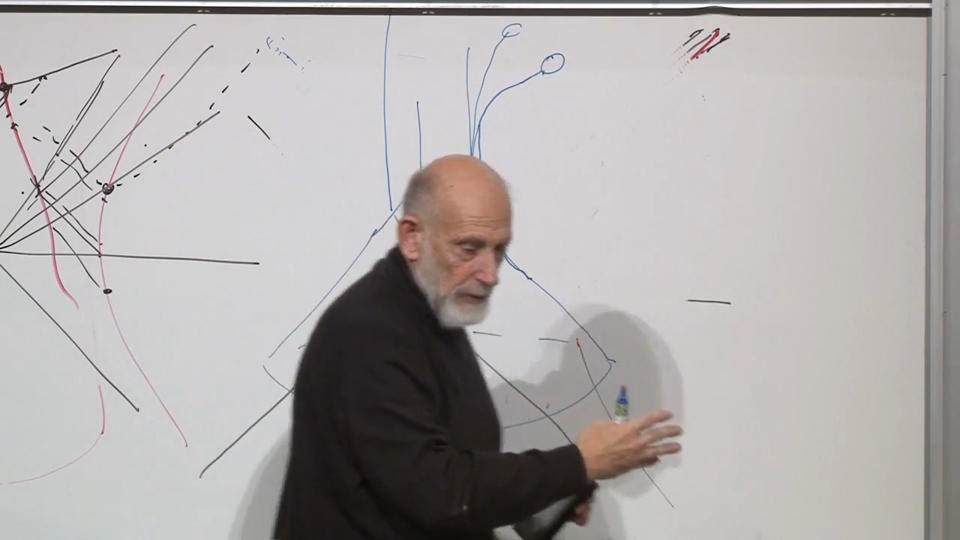
\includegraphics[width=0.90\textwidth]{lecture_06_figure_07.png}
\caption{一个坍缩的球壳，以及视界从中心向外增长以与它相遇。该图是下一讲中展开的全局坍缩几何的一个预览。}
\lectureframe{01:57:25}
\end{figure}

\begin{classroomqa}
\audiencequestion{如果在外部坐标时间中没有任何东西穿越视界，黑洞又如何能够形成或增长？}
\lecturerresponse{这个前提把一种坐标陈述与一种全局陈述混在了一起。坍缩的物质在有限的固有时内到达相关区域，而事件视界则由整个时空的因果结构决定。在球壳图景中，它从中心开始并向外增长以与球壳相遇。外部观测者所看到的延迟、红移的图景仍然与那个全局视界一致。
\lecturetimestamp{01:53:11--01:57:34}}
\end{classroomqa}

\section{两个球面之间的逃逸方向}

视界和光子球把光线问题划分为不同的情形。在半径
\begin{equation}
2MG<r<3MG,
\end{equation}
处，一条径向向外的光线可以逃逸到无穷远。一条切向光线则不能；它会向内下落。在这些方向之间存在一个逃逸锥。越靠近视界，该锥就越围绕向外的径向方向收窄。穿越视界之后，它完全闭合。

\begin{classroomqa}
\audiencequestion{位于视界与光子球之间的光源能否向外发送任何信号？}
\lecturerresponse{能。只要发射事件位于\(2MG\)之外，足够径向的向外零测地线就能逃逸。关于\(3MG\)内部角向运动向内落入的说法并不禁止径向逃逸。结果取决于发射方向，而随着光源接近视界，允许的向外锥面会变窄。
\lecturetimestamp{01:57:34--01:59:48}}
\end{classroomqa}

\begin{classroomqa}
\audiencequestion{从外部到达的光线能否穿过光子球内部、掉头并再次出现？}
\lecturerresponse{不能沿着所讨论类型的零测地线做到。掉头点将具有零径向速度，因此光线会在低于\(3MG\)的半径处瞬时切向；在那里角向轨迹向内落入，而不是掉头向外。然而，已经位于两个球面之间的光源可以在穿过视界之前发射足够径向的向外光线。
\lecturetimestamp{01:59:49--02:01:27}}
\end{classroomqa}

最后一个问题有意地不那么确定。设想Alice和Bob都被保持在视界之外的同一半径处。附近的观测者显然可以交换信号。如果他们围绕球面相距很远，那么直接的零路径及其极限角范围需要显式的测地线计算。课堂提出了一条间接路线：将信息几乎径向向外发送到更安全半径处的中继站，在那里携带它绕行，然后再向内发送回来。另一种版本让向外抛出的物体或信号掉头返回。这些路线说明了为什么切向圆轨道的失败本身并不禁止外部观测者之间的一切通信。

\begin{classroomqa}
\audiencequestion{两个悬停在相同近视界半径处的观测者能否绕过黑洞进行通信？}
\lecturerresponse{局部地，能。对于相距很远或正好相对的观测者，直接路径的极限在讲座中并未算出，不应被提升为定理。讨论首先将那个角向测地线问题留作未决，然后指出间接信号可以几乎径向向外发送，在较大半径处被中继绕行，然后返回。接近视界会使直接有用的角范围越来越窄，但在视界之外，向外路线仍然可用。
\lecturetimestamp{02:01:29--02:04:17}}
\end{classroomqa}

下一步是用坍缩天体的整体几何取代这些近视界草图，并精确地看到事件视界如何增长。